\documentclass[a4paper,english]{article}
\usepackage[utf8]{inputenc}
\usepackage[T1]{fontenc,url}
\usepackage{babel,textcomp}
\usepackage{graphicx, wrapfig}
\usepackage{graphics}
\graphicspath{
	{../figures/}
}
\usepackage{cite}
\usepackage{amsmath}
\usepackage{bm}
\usepackage{stackengine}
\usepackage{listings}
\usepackage{amsfonts}
\urlstyle {sf}
\title {Project 2 FYS-STK4155 Autumn 2018}
\author {Jon Audun Baar}
\begin{document}
\maketitle

%The last couple of years different machine learning techniques have
%gained enormous popularity due to several factors. 
%In this project we aim to
%evaluate the performance of these two methods on an often studied problem
%in physics.
%\par
%First we use both methods to predict the energy of the system. Then we 
%apply both methods over again to predict the phases of the systems.

\section*{Abstract}
In this project we compared regression analysis and neural networks as 
methods for developing models for both continuos and 
categorical data. 
We used data generated by the Ising model in both cases. 
First we showed that linear regression is prefferable over 
deep networks in our special case when it comes to 
learning efficiency. With a large amount of data they both 
created good models however. 
We then compared logistic regression and deep neural networks on 
a classification problem and showed that the neural net by far
is better than regression in this case due to the non-linear 
classification boundaries of our problem.

\section{Introduction}
%The one sentence about what machine learning is for the new guy.
The concept of machine learning have gained a hughe popularity boost over 
the last couple of years. And this is no wonder: the techniques 
have a wide range of applications and can be a major asset
if you know when to use what.
\par
When to use what is exactly what we're going to have a brief
peek into in this project. 
We aim to evaluate the performance of regression analysis and deep
neural networks in two different cases. 
First we compare linear regression and neural networks in the case 
of a continuous output, then we move on to comparing logistic regression
and neural nets in the case of a classification problem. 
In both cases we use the much studied Ising model to generate our datasets.

\section{Method}
In order to present the methods used, 
we first need to establish some terminology and notation. 
In this text we will use both machine learning terminology and more 
statistical language. Hence we talk about our independent variables both
as \textit{input} and \textit{predictors}, and our dependent 
variables as both \textit{output} and \textit{response}.
We assume that we are given a dataset consisting of 
$N \in \mathbb{N}$ samples, where each sample consists of $p\in\mathbb{N}$ 
input variables
and one output. We then denote by $x_{ij}$ the $j$-th predictor of
the $i$-th sample and by $t_i$ the response of the $i$-th sample. 
Further we partition the dataset into training data consisting of
$N_t$ samples, and test data consisting of $N_v$ samples. Of course we
then have $N_t + N_v = N$.
\par
When applying both regression analysis and neural 
networks the basic concept is the same:
You want to fit a model to your trainingdata by minimizing some sort of 
error. The model and minimization methods however are different.

\subsection{Regression analysis}
\subsubsection{Linear regression}
The concept of linear regression should by now be known from 
\cite{baarravndal}. 
The only difference in this project is that we now have $p=L$ predictors 
instead of $2$ and a fixed model instead of several different models
of different complexity. Since our model is given by
\begin{equation}
    E = \sum_{i,j=1}^L \bm{J}_{i,j} x_i x_j
\end{equation}
where $\bm{J}_{i,j}$ is the coupling constant from spin $i$ to spin $j$,
our design matrix is now given by
\begin{equation}\begin{split}
    X \ = \
    \begin{bmatrix}
        x_{1,1}x_{1,1} &\dots &x_{1,1} x_{1,L}
        &\dots
        &x_{1,L}x_{1,1}  &\dots &x_{1,L} x_{1,L} \\
        x_{2,1}x_{2,1}  &\dots &x_{2,1} x_{2,L}
        &\dots
        &x_{2,L}x_{2,1} &\dots &x_{2,L} x_{2,L} \\
        \vdots &&\vdots &&&&\vdots\\ 
        x_{N,1}x_{N,1} &\dots &x_{N,1} x_{N,L}
        &\dots
        &x_{N,L}x_{N,1} &\dots &x_{N,L} x_{N,L}
    \end{bmatrix}
\end{split}\end{equation}
Apart from this little twist the procedure is exactly the same as in 
\cite{baarravndal}.
\subsubsection{Logistic regression}
When the output of a dataset is categorical, logistic
regression is a possible method for developing a model for the 
relationship between input and output. 
The model to fit then gives us the probabilities for a datapoint to be of 
any of the given categories. In our case we have only two categories 
and our model is then given by
\begin{equation}
    p(\bm{x}_i; \beta_0, \bm{\beta}) 
    \ = \ \frac{1}{1 + \exp(- \beta_0 - \bm{x}_i\bm{\beta})}
\end{equation}
where 
$p_1(\bm{x}_i; \beta_0, \bm{\beta}) := p(\bm{x}_i; \beta_0, \bm{\beta})$ 
then is the probability 
for datapoint $i$ to be of category $1$, and 
$p_2(\bm{x}_i; \beta_0, \bm{\beta}) := 1 -p(\bm{x}_i; \beta_0, \bm{\beta})$ 
is the probability for the same datapoint to be of category $2$.
Here $\bm{x}_i \in \mathbb{R}^p$ is the input of datapoint $i$ given
as a row vector. 
$\beta_0 \in \mathbb{R}$ and $\beta \in \mathbb{R}^p$ (column vector) 
are the coefficients/weights of the model which we are to estimate.
\par
If we assume that the targets of the outputs of the model is 
$\{t_i\}_{i=1}^N$, the cost function is then given by 
\begin{equation}
    C(\beta_0, \bm{\beta}) \ = \
    \sum_{i=1}^N t_i \log(p(\bm{x}_i; \beta_0, \bm{\beta})) + 
    (1 - t_i) \log(1- p(\bm{x}_i; \beta_0, \bm{\beta}))
\end{equation}
where $\log$ is the natural logarithm.
\par
As opposed to some cases of linear regression, there is no analytical
solution to the problem of minimizing this cost function. We therefore
have to resort to numerical methods to approximate a minimum. This will
be discussed in section 2.3. Anyway we will need the gradient and Hessian
of $C$ in order to apply these methods. These are
\begin{equation}
    \nabla C(\beta_0, \bm{\beta}) \ = \
    \sum_{i=1}^N \bm{x}_i(t_i - p(\bm{x}_i; \beta_0, \bm{\beta}))
\end{equation}
and
\begin{equation}
    \frac{\partial^2 C(\beta_0, \bm{\beta})}
    {\partial \beta \partial \beta^T} \ = \
    - \sum_{i=1}^N \bm{x}_i \bm{x_i}^T 
    p(\bm{x}_i; \beta_0, \bm{\beta})(1 - p(\bm{x}_i; \beta_0, \bm{\beta}))
\end{equation}
respectively.

\subsection{Neural Networks}
When dealing with neural networks, the overarching concept is still the 
same as when one does regression analysis: We have a model that we wish 
to fit to a dataset by minimizing some error. The difference 
is the model and the methods by which we minimze the error.
\par
As the scope of this text is not to fully explain neural networks
rather than to analyse it's performance in some special cases, we will
simply establish the needed notation and assumptions. For a thorough
explanation of neural networks consult \cite{hastie_NN}.
\par
We will use a sequential multilayered network with $L$ layers as our model.
Let the number of nodes in layer $l$ be denoted by $n^l$ and let 
$n^0 = p$. We then denote
by $W^l \in \mathbb{R}^{n^l \times n^{l-1}}$ and 
$\bm{b}^l \in \mathbb{R}^{n^l}$ the weight matrix and bias 
vector of layer $l$ respectively. 
Finally we denote by $f^l: \mathbb{R}^{n^l} \rightarrow \mathbb{R}^{n^l}$ 
the activation function of 
layer $l$. As we in our case have a binary classification problem,
it is sufficient with one node in the last layer, and our model is then
given by $h: \mathbb{R}^p \rightarrow [0,1]$ defined by
\begin{equation}
    h(x) \ = \ f^L( \dots f^2(W^2 f^1(W^1 \bm{x} + \bm{b}^1) + \bm{b}^2) 
    + \dots + \bm{b}^L)
\end{equation}

%\subsubsection{Two different costfunctions}

%\subsubsection{Activation functions}

%\subsubsection{Activation functions}
There are several activationfunctions: Sigmoid, relu, softmax, 
leaky relu, tanh and
so on. Since we basicly are faced with a forest of parameters to tweak
when working with neural nets, we've limited ourselves to try out just a
few in this project.
%\begin{itemize}
%    \item
%        The \textbf{Sigmoid} function is given by 
%        \begin{equation}
%            f(z) = \frac{1}{1 + \exp(-z)}
%        \end{equation}
%    \item
%        \textbf{Relu}
%    \item
%        \textbf{Softmax}
%    \item
%        \textbf{tan h}
%\end{itemize}

\subsection{Gradient methods}
As we have now seen, there is no analytical solutuion to the problem
of minimizing the cost function when dealing with both logistic regression
and neural networks. For this reason we need to consider some numerical 
methods for approximating the minimium. All these methods have one 
weakness in common, they might end up finding local minima. However 
if the functions we are minimizing are convex, we are guaranteed to find
the global minima. Luckily most of the functions we are interested in
minimizing are convex. (If they are concave, the negative of the function
is concave and we can maximize this instead.)

\subsubsection{Gradient descent}
The perhaps simplest approach to minimizing a real valued function
$f$ iteratively, is to set some starting point $\bm{x}_0$, compute the gradient
$\nabla f$ in $\bm{x}_0$, and move $\eta > 0$ in the opposite direction of 
this gradient in order to obtain 
$\bm{x}_1 = \bm{x}_0 - \eta \nabla f(\bm{x}_0)$. Then
one iterates by setting 
$\bm{x}_{i+1} = \bm{x}_i - \eta \nabla f\bm{(}x_0)$. 
This is the framework of gradient descent.
For small enough $\eta$ this implies $f(\bm{x}_i) > f(\bm{x}_{i+1})$. 
The problem with this approach is to find out what 
$\eta$ is small enough. If we choose
$\eta$ too small, it might take days for our algorithm to converge. If 
we on the contrary choose $\eta$ to big, it might not converge at all.

\subsubsection{Newton-Raphson}
The Newton-Raphson method is a kind of gradient descent method, 
except we choose the learning rate in a more clever way. We thus 
start out by choosing a random starting point $\bm{x}_0$, just as in the 
case of gradient descent. The update step however is a bit different:
\begin{equation}
    \bm{x}_{i+1} \ = \ \bm{x}_{i} - 
    \frac{\partial^2 f(\bm{x}_i)}{\partial \bm{x}_i \partial \bm{x}_i^T} 
    \frac{\partial f(\bm{x}_i)}{\partial \bm{x}_i}
\end{equation}
The result is a method that converges way faster than normal gradient 
descent. The draw back is however the need to compute the Hessian of 
your objective function. For a thourough derivation of this method 
consult \cite{gradient}

\subsubsection{Stochastic gradient descent}
To avoid overfitting when training neural networks, training on 
randomly picked batches of the training data for each iteration is a good
regularization method. If we let $b$ be our batch size, the first step of
this method consists of dividing the training data into $N//b$ batches. 
One does this by picking from the $N$ data-points without replacement. 
The second step is then to perform a gradient descent as described in 
section 2.3.1 with a new batch for each iteration.

\subsection{Performance measures}
\subsubsection{MSE, R2-score, Bias and Variance}
For an explanation of the MSE, R2-score, bias and variance please
consult \cite{baarravndal}.
\subsubsection{Accuracy score}
For classification problems with multiple categories the performance
measures we derived in \cite{baarravndal} is not well defined.
Therefore in order to measure the performance of our classification models,
we define the following measure
\begin{equation}
    \text{Accuracy} = 1/N \sum_{i=1}^N \chi_{\{t_i\}}(y_i)
\end{equation}
where $\chi_{\{t_i\}}$ is the indicator function for the set
$\{t_i\}$ and $y_i$ is the class predicted by our model. 
In other words, the accuracy is the ratio of correct classifications 
over the total number of classifications.

\subsection{The Ising model}
The model we use to generate data for our experiments is the well known
Ising model given by
\begin{equation}
    E \ = \ - J \sum_{\langle kl \rangle}^N s_k s_l
\end{equation}
where $\langle kl \rangle$ indicates that we sum only over neighbouring
spins, 
$s_k = \pm 1$ are the spin values, $N$ is the total number of spins and $J$ is the coupling 
constant that expresses the strength of the interaction between 
neighbouring spins. For a more thorough explanation of this model
consult \cite{ising}.

\section{Implementation}
Implementation of the logsitic regression and neural networks was done 
with Python. We've chosen to implement each of the models as classes. 
The full code with test is located at 
https://github.com/jonabaa/Project2.git

\section{Analysis of the methods}
\subsection{Estimating the coupling constant of the one-dimensional 
Ising model using linear regression}
We investigated how well OLS-, Ridge- and Lasso regression were able
to estimate the couplingconstants 
of the general Ising model 
given the spins $\bm{x}_i$ and the energies $E_i$ from
the onedimensional version of the model. We denote the coupling constants
of the general Ising model by $\bm{J}$.
None of the methods yielded useable models before $N_t$ was larger than
$200$, hence we used $N_t=400$ (and $N_v=600$) in our further
investigations. 

%We should look at different dataset sizes
%because it seems like Lasso is the first one to perfrom, and then 
%the other ones follow, BUT the coiplingconstants are best estimated
%by Lasso still for high numbers of samples. that is 2000.
\par
As one can see from figure 1, Lasso regression with 
$10^{-3} < \lambda < 10^{-1}$ clearly outperforms the two other methods
in estimating the coupling constants. This is further established
by the plots in figure 2.
\begin{figure}
    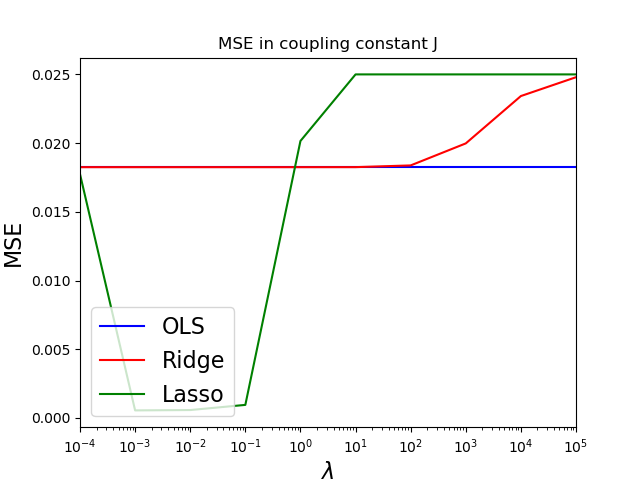
\includegraphics[scale=.7]{MSE_J_N1000_train4test6.png}
    \caption{Comparing coupling constants}
\end{figure}

\subsection{Estimating the energy of the one-dimensional 
Ising model using deep neural networks}
We performed a grid search over the regularization parameter $\lambda$
and the size of the training data set. This showed that 
neural networks can do very well predicting enrgies, 
with R2-scores exceeding $99\%$. The only draw back is the need for 
large amounts of datapoints for training. 
%As the plot suggests we
%need roughly ten to hundred times as much data as when using
%lasso regression.

\subsection{Determining the phase of the two-dimensional Ising model using
logistic regression}
For as large datasets as my computer could handle, logistic regression
performed poorly consistently. Mininmizing the cost function with 
Newton-Raphson tended to yield the fastest and best results, yet
not good results. We managed to get an accuracy of roughly $70\%$ 
for $N=3000$. 

\subsection{Determining the phase of the two-dimensional Ising model using
deep neural networks}
Classification seems to be some of the strengths of neural networks, at
least in this case. We did a grid search over different regularization
paramters and training data sizes and managed to make models that
predicted with accuracys well over $97\%$, which must be considered to
be very good.

\section{Conclusion}
The clearest result from this investigation would be that logistic
regression don't perform well in the case of classifying wether a spin
configuration is stable or unstable. Deep neural networks, on the contrary,
performs the task of classification very well.
\par
It is also pretty obvious from figure 2 that Lasso regressoion is the 
only method that yields good results in estimating the coupling constants
in the Ising problem.
\bibliography{references}{}
\bibliographystyle{plain}
\end{document}
